\chapter{MLFlow – An easy way of Managing and Monitoring Training}

%==============================================================================
%
%==============================================================================
\section{Introduction to MLFlow}

Machine learning workflows often involve repeated training runs with slightly different hyperparameters, code versions, and datasets. Without proper tracking, this becomes chaotic — especially in collaborative or operational environments. MLFlow provides a robust solution for managing this complexity by organizing experiments and tracking key information throughout the machine learning lifecycle.

\begin{figure}[htbp]
    \centering
    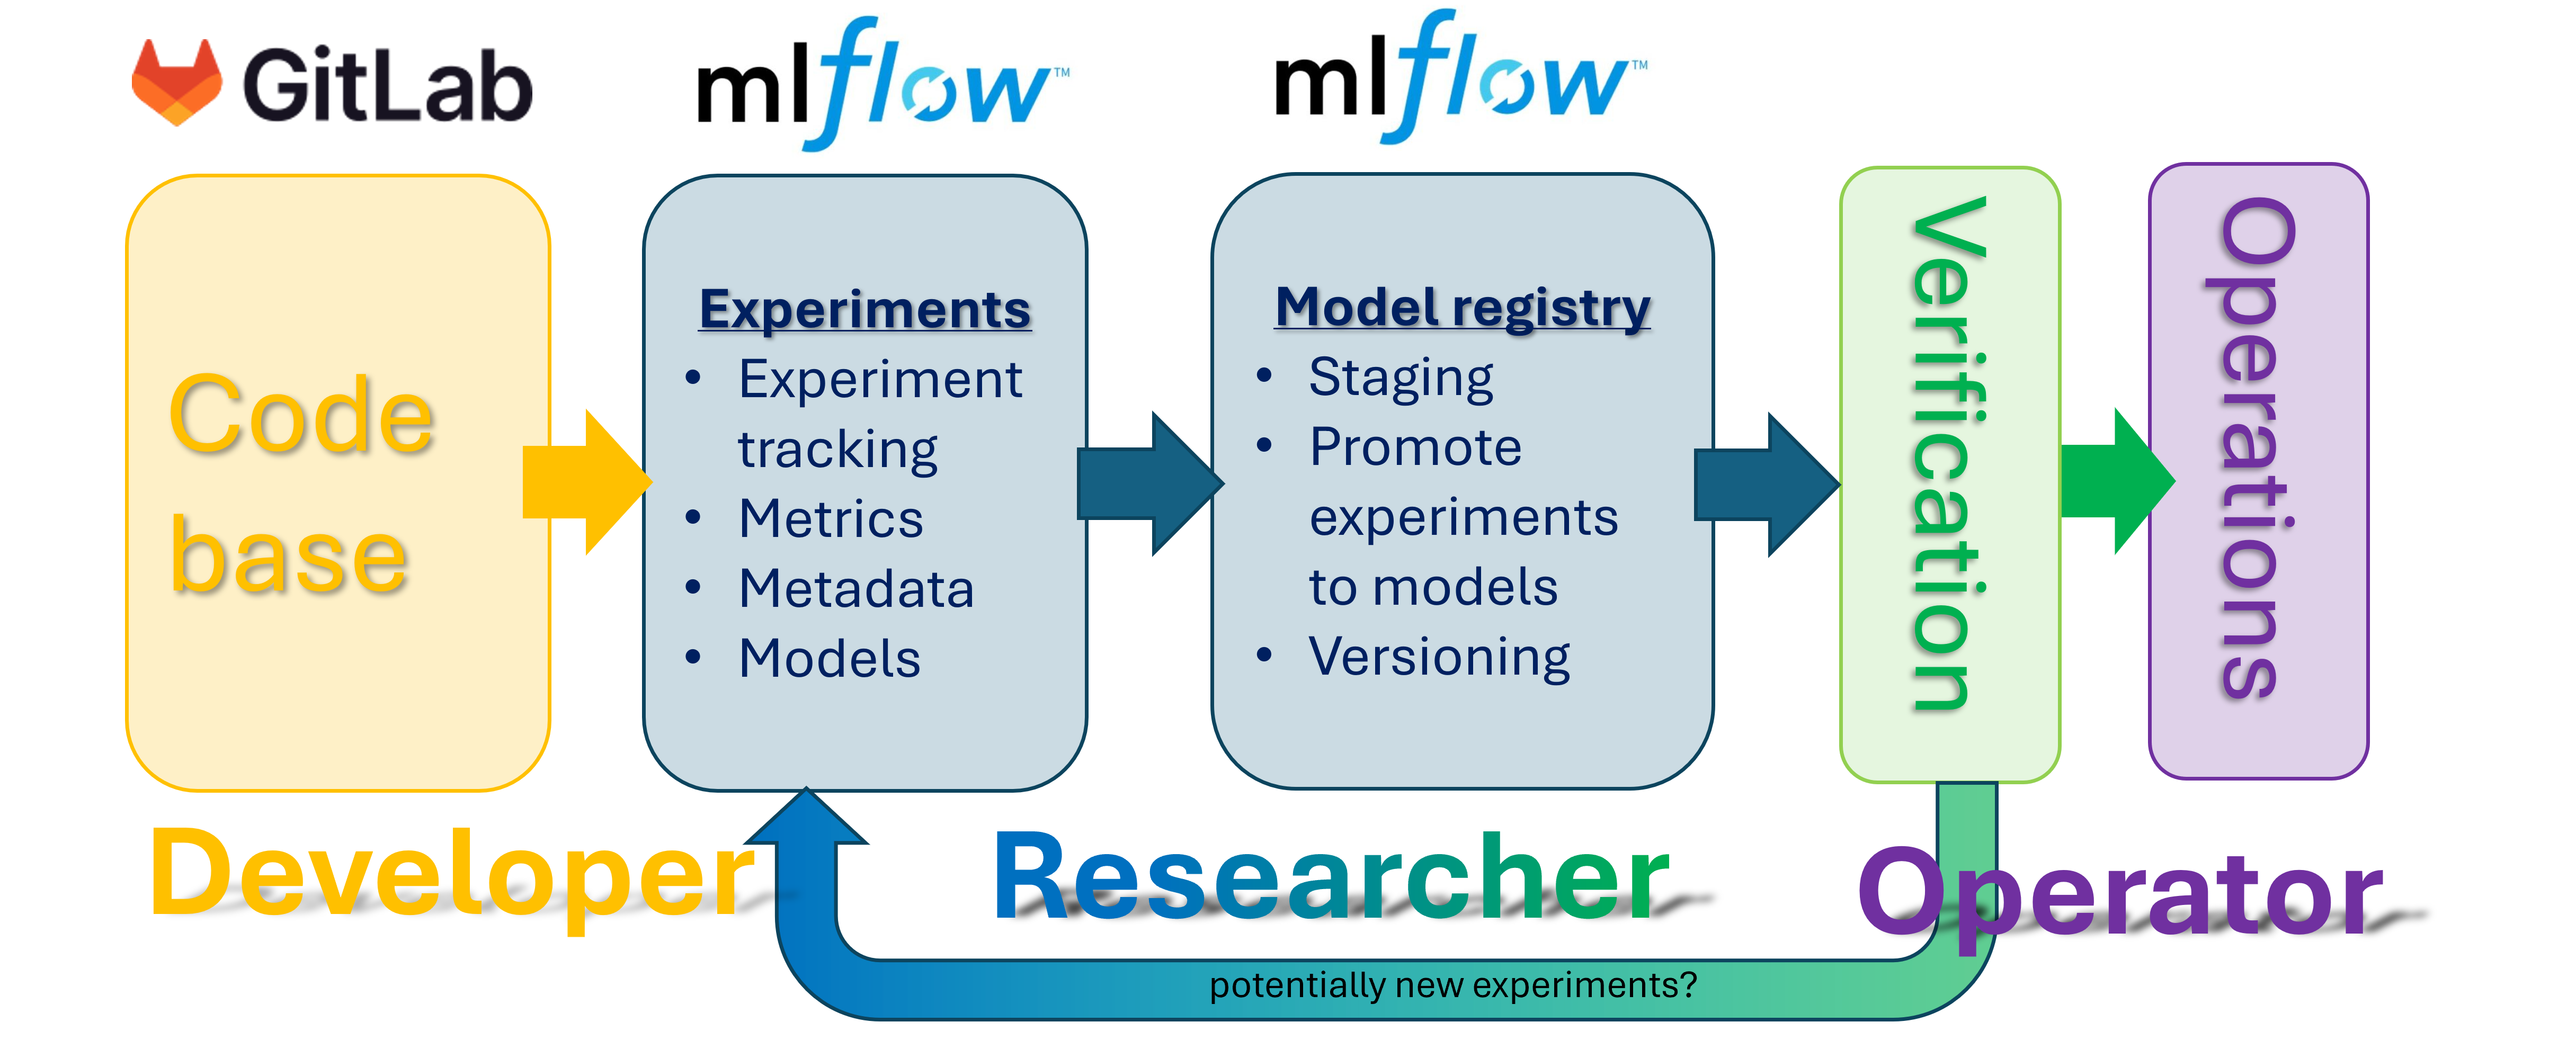
\includegraphics[width=0.95\textwidth]{images/mlflow_flow.png}
    \caption{MLFlow in an MLOps pipeline: The workflow illustrates how developers, researchers, and operators interact through MLFlow. Experiments are tracked, metrics and models are stored, and selected runs can be promoted to the model registry. Verified models are deployed to operations, and outcomes can lead to new experiments.}
    \label{fig:mlflow_pipeline}
\end{figure}


\subsection{What is MLFlow?}

MLFlow is an open-source platform that addresses four primary functions of the machine learning workflow:

\begin{itemize}
    \item \textbf{Tracking:} Log parameters, metrics, artifacts, and code versions.
    \item \textbf{Projects:} Package ML code in a reusable and reproducible form.
    \item \textbf{Models:} Manage and deploy different versions of trained models.
    \item \textbf{Recipes:} Automate and standardize training pipelines.
\end{itemize}

In this chapter, we focus mainly on the \textbf{Tracking} and \textbf{Model Management} capabilities.

\begin{figure}[htbp]
    \centering
    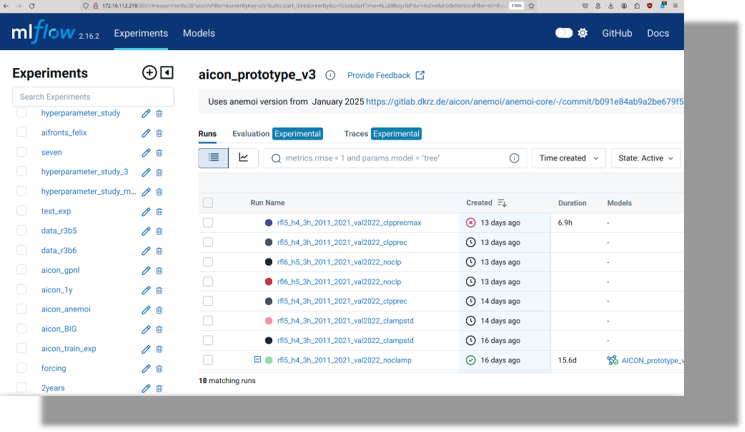
\includegraphics[width=0.85\textwidth]{images/MLFlow.png}
    \caption{MLFlow Web UI displaying logged experiments, parameters, and metrics.}
    \label{fig:mlflow_ui}
\end{figure}

%------------------------------------------------------------------------------
%
%------------------------------------------------------------------------------
\subsection{Why Do We Need Experiment Tracking?}

The need for reproducibility and transparency in ML pipelines is growing. Consider the following recurring challenges:

\begin{itemize}
    \item You forget which dataset was used to train a model.
    \item The best-performing parameter settings are lost or overwritten.
    \item Colleagues cannot reproduce your results.
    \item Operational users request model metadata, but it is not documented.
\end{itemize}

MLFlow provides solutions to these problems by creating a structured history of all your training runs.

%------------------------------------------------------------------------------
%
%------------------------------------------------------------------------------
\subsection{Core Concepts of MLFlow}

MLFlow Tracking organizes your work using the Experiment-Run hierarchy:

\begin{itemize}
    \item \textbf{Experiment:} A named collection of related training runs.
    \item \textbf{Run:} A single execution of training code, where parameters, metrics, and artifacts are logged.
\end{itemize}

Each run can store
\begin{itemize}
    \item \textbf{(Hyper-)Parameter:} settings of the experiments such as numeric values and strings,
    \item \textbf{Metrics:} values such as losses and scores that can be logged with each training step and epoch,
    \item \textbf{System Metrics:} step/epoch-dependent metrics of the system such as CPU usage and memory usage, and
    \item \textbf{Artifacts:} files such as plots or trained models.
\end{itemize}
MLFlow offers an interactive user interface to plot an compare different metrics within and across different training runs (Figs. \ref{fig:mlflow_boxplot}, \ref{fig:mlflow_contour}, \ref{fig:mlflow_metrics_2}). The metrics can even be analysed while the training is still running.

Each run is recorded either locally or on a remote tracking server, and can be explored visually using the MLFlow Web UI.
The tracking target is defined by the \textbf{Tracking URI}.


\begin{figure}[htbp]
    \centering
    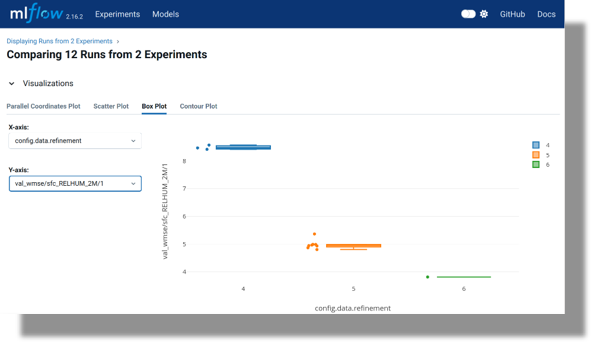
\includegraphics[width=0.85\textwidth]{images/mlflow03.png}
    \caption{Box Plot Comparison in MLFlow: Model runs from different experiments are compared based on a validation metric, with color-coded configurations. This helps identify parameter influences.}
    \label{fig:mlflow_boxplot}
\end{figure}

%------------------------------------------------------------------------------
%
%------------------------------------------------------------------------------
\subsection{Installing MLFlow}

You can install MLFlow using \texttt{pip}:

\begin{codeonly}{Install MLFlow}
pip install mlflow
\end{codeonly}

It is recommended to use a virtual Python environment to isolate dependencies.

\begin{figure}[htbp]
    \centering
    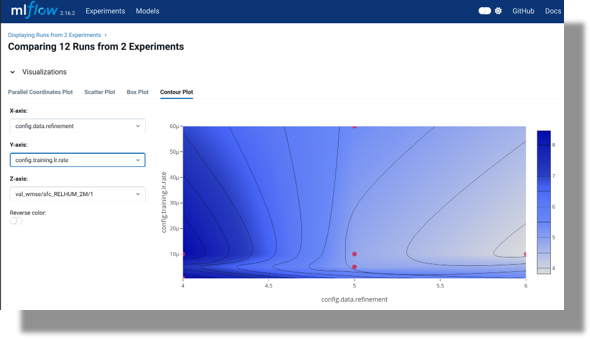
\includegraphics[width=0.85\textwidth]{images/mlflow04.png}
    \caption{Contour Plot Visualization in MLFlow: Visualization of the effect of two hyperparameters on a performance metric. The color gradient highlights optimal regions for tuning.}
    \label{fig:mlflow_contour}
\end{figure}

%------------------------------------------------------------------------------
%
%------------------------------------------------------------------------------
\subsection{Basic Logging Example}

The following Python code demonstrates how to log an experiment using MLFlow:

\begin{codeonly}{Minimal MLFlow Logging}
import mlflow

mlflow.set_experiment("MyFirstExperiment")

with mlflow.start_run(run_name="initial_run"):
    mlflow.log_param("learning_rate", 0.001)
    mlflow.log_metric("loss", 0.256)
\end{codeonly}

This code snippet performs the following:
\begin{itemize}
    \item Creates or reuses an experiment called \texttt{MyFirstExperiment}.
    \item Starts a run named \texttt{initial\_run}.
    \item Logs a hyperparameter and a metric to that run.
\end{itemize}

%------------------------------------------------------------------------------
%
%------------------------------------------------------------------------------
\subsection{Launching the MLFlow Web Interface}

Once an experiment has been logged, you can start a local web interface with:

\begin{codeonly}{Start MLFlow UI}
mlflow ui
\end{codeonly}

By default, this opens a dashboard at \texttt{http://localhost:5000}, where you can explore experiments, compare runs, and visualize metrics or parameters.

%------------------------------------------------------------------------------
%
%------------------------------------------------------------------------------
\subsection{Summary}

MLFlow is a powerful tool to:

\begin{itemize}
    \item Organize and record training runs
    \item Compare performance between experiments
    \item Make machine learning more reproducible
    \item Share and manage models in a structured way
\end{itemize}

In the following sections, we will explore how to use MLFlow to log a complete neural network training process and how to run an MLFlow server for team collaboration.

%==============================================================================
%
%==============================================================================
\section{Logging ML Experiments with MLFlow}

In this section, we demonstrate the use of MLFlow in a real training scenario. The example implements a neural network that learns to predict wind chill based on temperature and wind speed, and logs the experiment to an MLFlow server.

%------------------------------------------------------------------------------
%
%------------------------------------------------------------------------------
\subsection{Preparing the Environment}

Make sure MLFlow is installed and your server is running (local or remote).

\begin{codeonly}{Install MLFlow}
pip install mlflow
\end{codeonly}

Then configure the tracking URI and the experiment name.

\begin{codeonly}{Setup an Experiment}
import mlflow

mlflow.set_tracking_uri(uri="http://localhost:5000")
mlflow.set_experiment("Wind Chill Example")
\end{codeonly}

This sets up logging to a local MLFlow server and defines the experiment under which training runs are grouped.

%------------------------------------------------------------------------------
%
%------------------------------------------------------------------------------
\subsection{Generating Synthetic Data}

We simulate temperature and wind speed data, and compute wind chill values using a standard formula:

\begin{codeonly}{Generate Data}
import numpy as np
import torch

tt = np.random.uniform(-20, 10, 500)   # Temperature in Celsius
ff = np.random.uniform(0, 50, 500)     # Wind speed in km/h

wc = 13.12 + 0.6215 * tt - 11.37 * (ff ** 0.16) + 0.3965 * tt * (ff ** 0.16)

x_train = torch.tensor(np.column_stack((tt, ff)), dtype=torch.float32)
y_train = torch.tensor(wc, dtype=torch.float32).view(-1, 1)
\end{codeonly}

This data is used to train a regression model.

%------------------------------------------------------------------------------
%
%------------------------------------------------------------------------------
\subsection{Defining the Model}

We use a simple feedforward neural network with two hidden layers:

\begin{codeonly}{Wind Chill Model}
import torch.nn as nn

class wind_chill_model(nn.Module):
    def __init__(self, hidden_dim):
        super().__init__()
        self.fc1 = nn.Linear(2, hidden_dim)
        self.fc2 = nn.Linear(hidden_dim, hidden_dim)
        self.fc3 = nn.Linear(hidden_dim, 1)
        self.relu = nn.ReLU()

    def forward(self, x):
        x = self.relu(self.fc1(x))  # layer 1
        x = self.relu(self.fc2(x))  # layer 2
        return self.fc3(x)
\end{codeonly}

%------------------------------------------------------------------------------
%
%------------------------------------------------------------------------------
\subsection{Training the Model with MLFlow Logging}

The training process logs parameters and metrics using MLFlow.

\begin{codeonly}{Train and Log}
hidden_dim = 20
model = wind_chill_model(hidden_dim=hidden_dim)
criterion = nn.MSELoss()
optimizer = torch.optim.Adam(model.parameters(), lr=0.0005)

with mlflow.start_run(run_name="logging 01"):
    mlflow.log_param("hidden_dim", hidden_dim)

    for epoch in range(10000):
        model.train()
        optimizer.zero_grad()
        y_pred = model(x_train)
        loss = criterion(y_pred, y_train)
        loss.backward()
        optimizer.step()

        if (epoch + 1) % 500 == 0:
            mlflow.log_metric("loss", loss.item(), step=epoch)
\end{codeonly}

The log includes both parameter settings and evolving loss values.
To harness the full potential of MLflow, one should log all metrics including \texttt{lr} in this example.

%------------------------------------------------------------------------------
%
%------------------------------------------------------------------------------
\subsection{Logging Plots and the Final Model}

After training, we log a loss curve and the final model.

\begin{codeonly}{Log Artifacts}
import matplotlib.pyplot as plt

plt.plot(train_loss, label="training loss")
plt.yscale('log')
plt.xlabel("epoch")
plt.ylabel("loss")
plt.legend()
plt.tight_layout()
mlflow.log_figure(plt.gcf(), "figure.png")

from mlflow.models import infer_signature
signature = infer_signature(x_train.numpy(), model(x_train).detach().numpy())
mlflow.pytorch.log_model(model, "model", signature=signature)
\end{codeonly}

Artifacts such as loss curves and model binaries appear in the MLFlow UI and can be downloaded or registered.

%------------------------------------------------------------------------------
%
%------------------------------------------------------------------------------
\subsection{Results in the MLFlow UI}

You can explore the run in the web interface while its running or afterwards. Just open your browser, type \texttt{localhost:5000} and you will be able to inspect your example. The loss curve is visible under the \textit{Metrics} tab, and the model is listed under \textit{Artifacts}. Depending on the MLFlow version, there is a metrics tab either at the main window or after you chose the experiments.

\begin{figure}[htbp]
    \centering
    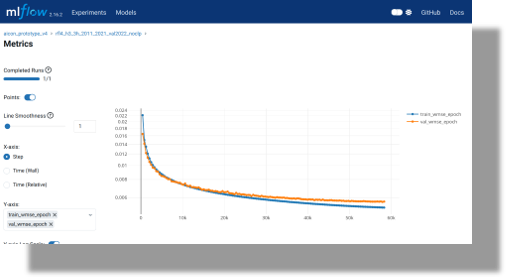
\includegraphics[width=0.85\textwidth]{images/mlflow01.png}
    \caption{MLFlow Metrics View: The training and validation losses over time are automatically visualized.}
    \label{fig:mlflow_metrics_2}
\end{figure}

\begin{figure}[htbp]
    \centering
    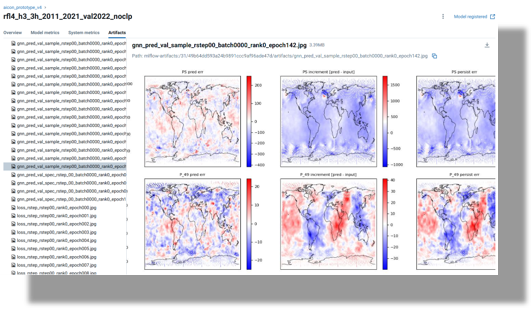
\includegraphics[width=0.85\textwidth]{images/mlflow02.png}
    \caption{MLFlow Artifact Browser: Logged outputs such as loss plots and models appear here and can be downloaded.}
    \label{fig:mlflow_artifacts_2}
\end{figure}

%------------------------------------------------------------------------------
%
%------------------------------------------------------------------------------
\subsection{Summary}

In this section, we demonstrated:

\begin{itemize}
    \item Creating a synthetic dataset and training a model
    \item Logging model parameters, metrics, and artifacts with MLFlow
    \item Visualizing results through the MLFlow UI
\end{itemize}

This forms the basis for more complex tracking and collaborative workflows, which we explore in the next section.

%==============================================================================
%
%==============================================================================
\section{Running an MLFlow Server}

While local logging to a directory is useful for experimentation, a shared MLFlow server is essential for team collaboration. In this section, we show how to start MLFlow in both local and multi-user network modes, and explain credential setup and deployment options.

%------------------------------------------------------------------------------
%
%------------------------------------------------------------------------------
\subsection{Starting the Local Web UI}

You can launch the built-in web interface with a simple command:

\begin{codeonly}{Start MLFlow UI}
mlflow ui
\end{codeonly}

This opens a browser window at \texttt{http://localhost:5000} displaying all logs from the default \texttt{mlruns/} directory.

\begin{figure}[htbp]
    \centering
    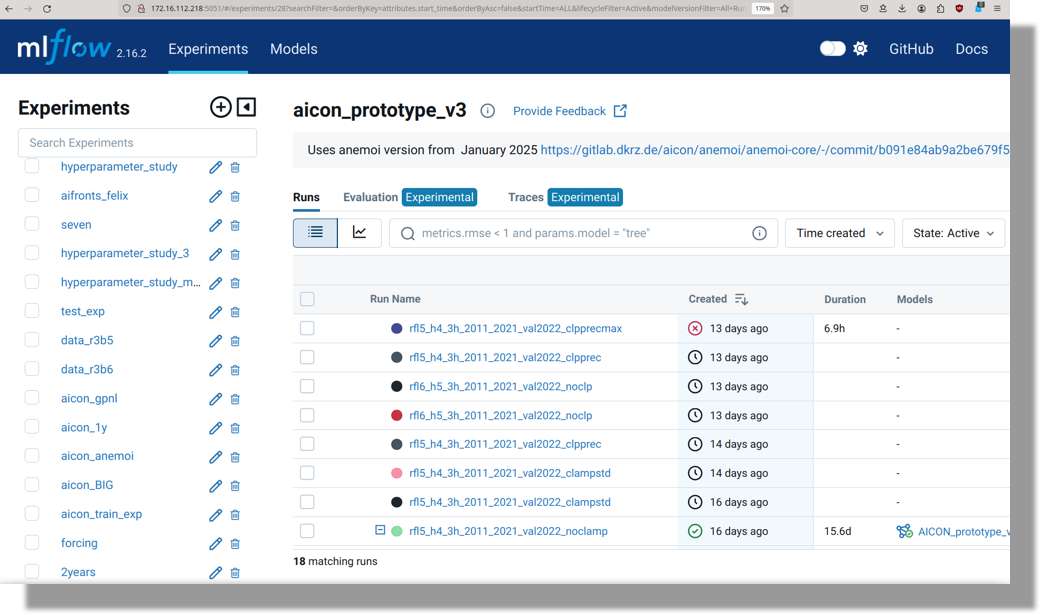
\includegraphics[width=0.85\textwidth]{images/mlflow_ui_local.png}
    \caption{MLFlow Web UI in local mode: Logs from \texttt{mlruns/} are visualized through a local server.}
    \label{fig:mlflow_local_ui}
\end{figure}

%------------------------------------------------------------------------------
\subsection{Launching a Stand-alone Server}

To share results across users or machines, launch MLFlow in \textbf{server mode}.
So far, port 5000 was restricted to users on the local system.
The following command binds MLFlow to all network interfaces so others can access your MLFlow server via the network.

\begin{codeonly}{Start MLFlow Server}
	mlflow server --host 0.0.0.0 --port 5000
\end{codeonly}

To keep the MLflow server running after starting it, you can launch it in the background using standard shell tools:

\begin{codeonly}{Shell background execution}
	mlflow server --host 0.0.0.0 --port 5000 &
\end{codeonly}

This appends an \texttt{\&}, sending the process to the background. However, it will stop if the terminal is closed. To make the server survive logout or disconnection, use \texttt{nohup}:

\begin{codeonly}{Detached execution using nohup}
	nohup mlflow server --host 0.0.0.0 --port 5000 > mlflow.log 2>&1 &
\end{codeonly}

This redirects all output to \texttt{mlflow.log} and keeps the process running independently of your shell session.


%------------------------------------------------------------------------------
%
%------------------------------------------------------------------------------
\subsection{Using Screen for Detached Execution}

\texttt{screen} is a terminal multiplexer that allows you to run processes in a separate session, which remains active even after you close your terminal. It is especially useful for long-running tasks like the MLflow server, where you may want to reconnect later to monitor logs or restart the process.

The following Bash script starts the MLFlow server inside a named GNU screen session.

\begin{codeonly}{Run MLFlow In Screen}
#!/usr/bin/env bash
screen -dmS mlflow
screen -S mlflow -X stuff "mlflow server --host 0.0.0.0 --port 5000\r"
\end{codeonly}

This allows the process to run in the background and be detached/re-attached.

%------------------------------------------------------------------------------
%
%------------------------------------------------------------------------------
\subsection{Credential and Authentication Setup}

MLFlow supports experimental basic authentication.
You might need to pip install the additional \texttt{auth} dependencies.
Define users in an auth config file and export its path:

\begin{codeonly}{Install auth and set MLFlow Auth}
pip install --upgrade "mlflow[auth,extras]"
export MLFLOW_AUTH_CONFIG_PATH="${PWD}/auth_config.ini"
export MLFLOW_FLASK_SERVER_SECRET_KEY=$(pwgen 32 1) # a random key
\end{codeonly}

On the server side, the initial admin user and password must be set together with other settings in \texttt{auth\_config.ini}:

\begin{codeonly}{Server-side configuration for basic auth in \texttt{\${PWD}/auth\_config.ini}}
[mlflow]
auth_enabled = true
database_uri = sqlite:///mlflow_auth.db
default_permission = READ
admin_username = admin
admin_password = ChangeThisPassword123!

[auth]
backend = basic
\end{codeonly}

Start the server with the \texttt{--app-name basic-auth } option:
\begin{codeonly}{Run MLflow server with basic auth}
    export MLFLOW_AUTH_CONFIG_PATH="${PWD}/auth_config.ini"
    mlflow server --host 0.0.0.0 --port 5000 --app-name basic-auth
\end{codeonly}

MLflow UI provides a simple page for creating new users at \texttt{<tracking\_uri>/signup}. Passwords can be managed with the Python API.

\begin{codeonly}{Change Password Via API}
from mlflow.server import get_app_client
auth = get_app_client("basic-auth", tracking_uri="http://localhost:5000")
auth.update_user_password("admin", "new_password") # Note that this code is stored in clear text.
\end{codeonly}

\begin{figure}[htbp]
    \centering
    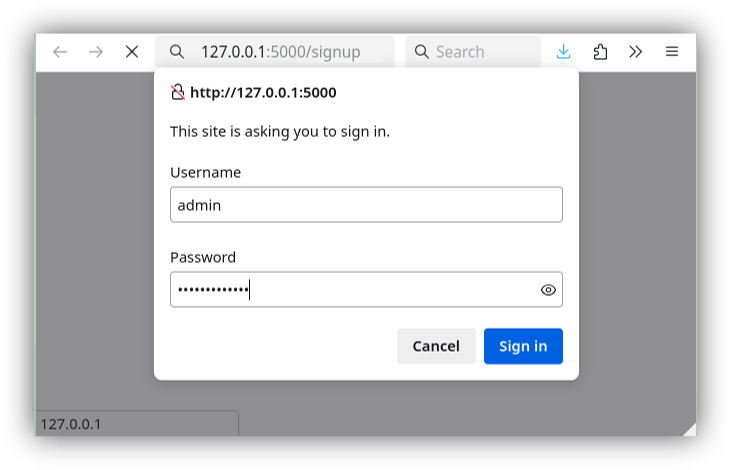
\includegraphics[width=0.85\textwidth]{images/mlflow_auth.png}
    \caption{MLFlow server started with basic auth. Users can log in later and inspect output or restart the service.}
    \label{fig:mlflow_auth}
\end{figure}

%------------------------------------------------------------------------------
%
%------------------------------------------------------------------------------
\subsection{User Credential File Setup}

To avoid typing credentials every time, store them in a private configuration file.

\begin{codeonly}{MLFlow Credential File \texttt{~/.mlflow/credentials}}
[mlflow]
mlflow_tracking_username = admin
mlflow_tracking_password = mysecret
\end{codeonly}

Make sure this file has strict access permissions:

\begin{codeonly}{Restrict Permissions}
chmod 600 ~/.mlflow/credentials
\end{codeonly}

The example script \texttt{code/code13/mlflow\_setup.py} provides a convenient command line interface to update and store your password on disk.
Please note that the password is stored unencrypted.

\begin{figure}[htbp]
    \centering
    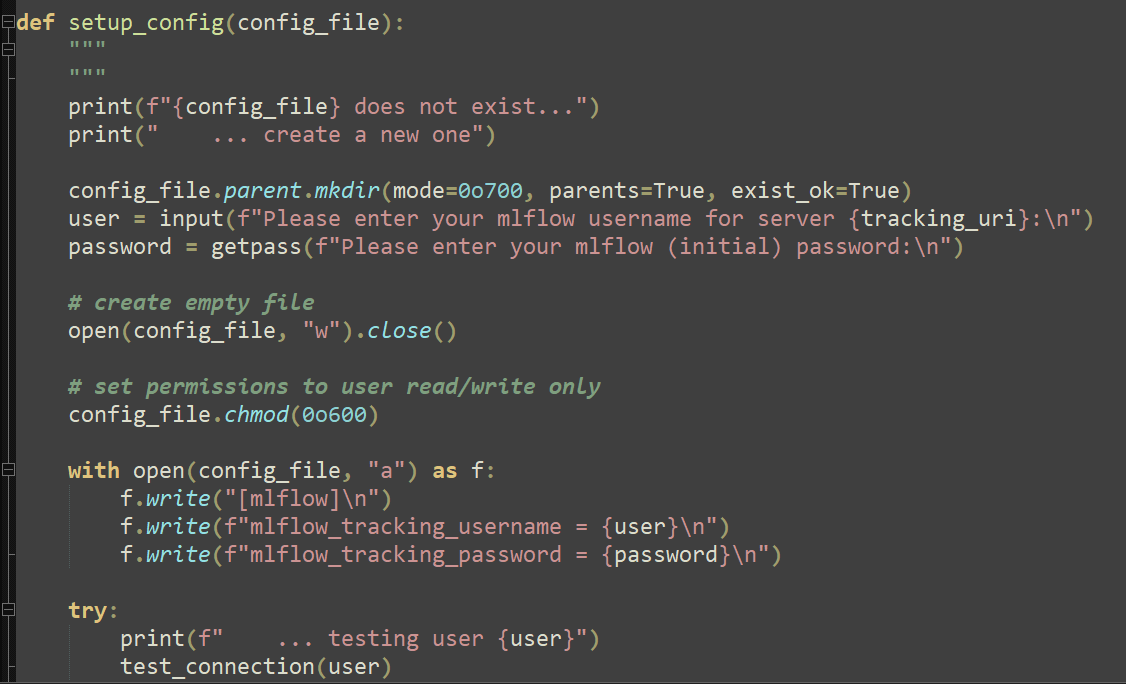
\includegraphics[width=0.85\textwidth]{images/mlflow_credentials.png}
    \caption{MLFlow credential storage in \texttt{\textasciitilde/.mlflow/credentials}, used by the Python client to access a secured MLFlow server.}
    \label{fig:mlflow_credentials}
\end{figure}

%------------------------------------------------------------------------------
%
%------------------------------------------------------------------------------
\subsection{Storage Backends and Performance}

By default, MLFlow uses the local file system as both metadata and artifact store. For larger setups, you can configure:

\begin{itemize}
    \item \textbf{Backend store}: SQLite, PostgreSQL, MySQL (for metrics, params)
    \item \textbf{Artifact store}: Local, NFS, S3, Azure Blob (for models, images)
\end{itemize}


Example:

\begin{codeonly}{Run Server With Custom Stores}
mlflow server \\
  --backend-store-uri sqlite:///mlflow.db \\
  --artifacts-destination ./mlflow-artifacts \\
  --host 0.0.0.0 --port 5000
\end{codeonly}

This setup is essential for reliable multi-user environments.

\begin{figure}[htbp]
    \centering
    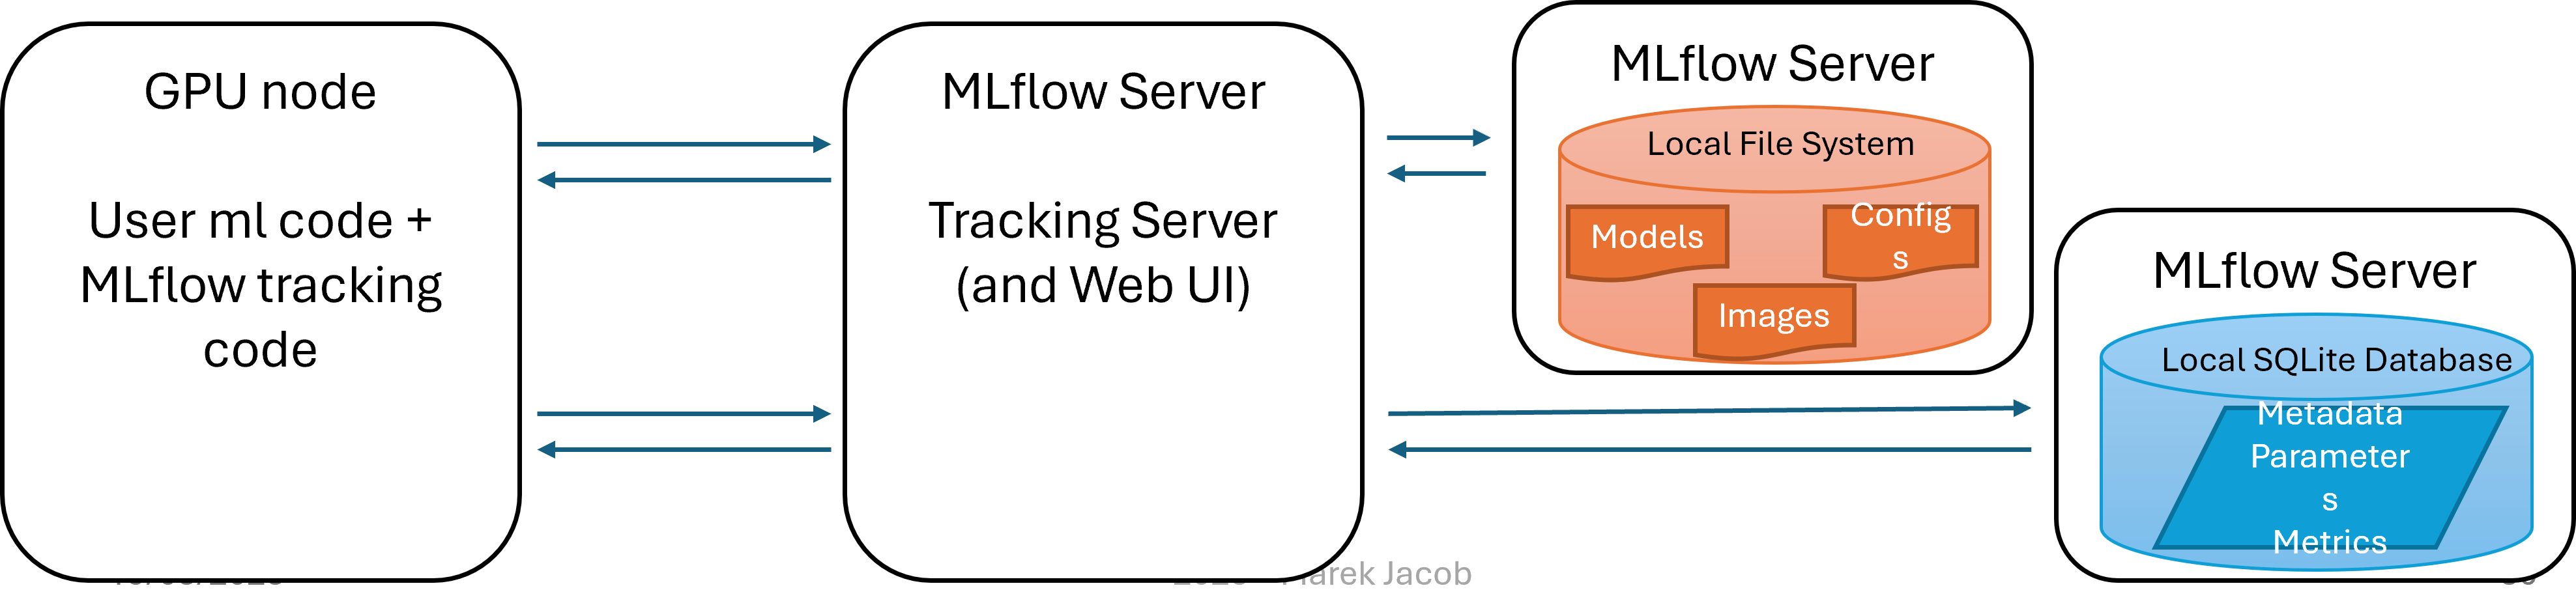
\includegraphics[width=0.85\textwidth]{images/mlflow_server_setup.png}
    \caption{Server Setup, with local storage and SQLite Database}
    \label{fig:mlflow_auth}
\end{figure}

%------------------------------------------------------------------------------
%
%------------------------------------------------------------------------------
\subsection{Summary}

We explored three MLFlow deployment modes:

\begin{itemize}
    \item \textbf{Local UI and server mode} using \texttt{mlflow ui}\footnote{\texttt{mlflow ui} aliases to \texttt{mlflow server}. Both commands do the same.}
    \item \textbf{Network server mode} using \texttt{mlflow server --host 0.0.0.0}
    \item \textbf{Multi-user mode} with authentication and background execution
\end{itemize}

These enable collaborative logging, secure experiment tracking, and long-running ML pipelines.



%==============================================================================
%
%==============================================================================
\section{Advanced Features and Model Management}

MLFlow is not limited to tracking metrics and saving plots. It also supports advanced workflows for model registration, cross-system migration of experiments, and deployment. This section covers the most useful tools for organizing and managing models in a production-like setting.

%------------------------------------------------------------------------------
%
%------------------------------------------------------------------------------
\subsection{Model Registry and Promotion}

MLFlow’s model registry allows you to store trained models in a central location, version them, and assign them lifecycle stages such as \texttt{Staging} or \texttt{Production}.

Each registered model version is associated with a specific run and its parameters, metrics, and artifacts. This enables full traceability.

\begin{itemize}
    \item Register a model at the end of a run
    \item Add tags and descriptions for each version
    \item Promote models to \texttt{Production} or \texttt{Archived}
    \item Roll back to earlier versions if needed
\end{itemize}

\begin{codeonly}{Register Model}
import mlflow
import mlflow.pytorch

with mlflow.start_run():
    ...
    mlflow.pytorch.log_model(model, "model")
    result = mlflow.register_model("runs:/{run_id}/model", "WindChillModel")
\end{codeonly}

\begin{figure}[htbp]
    \centering
    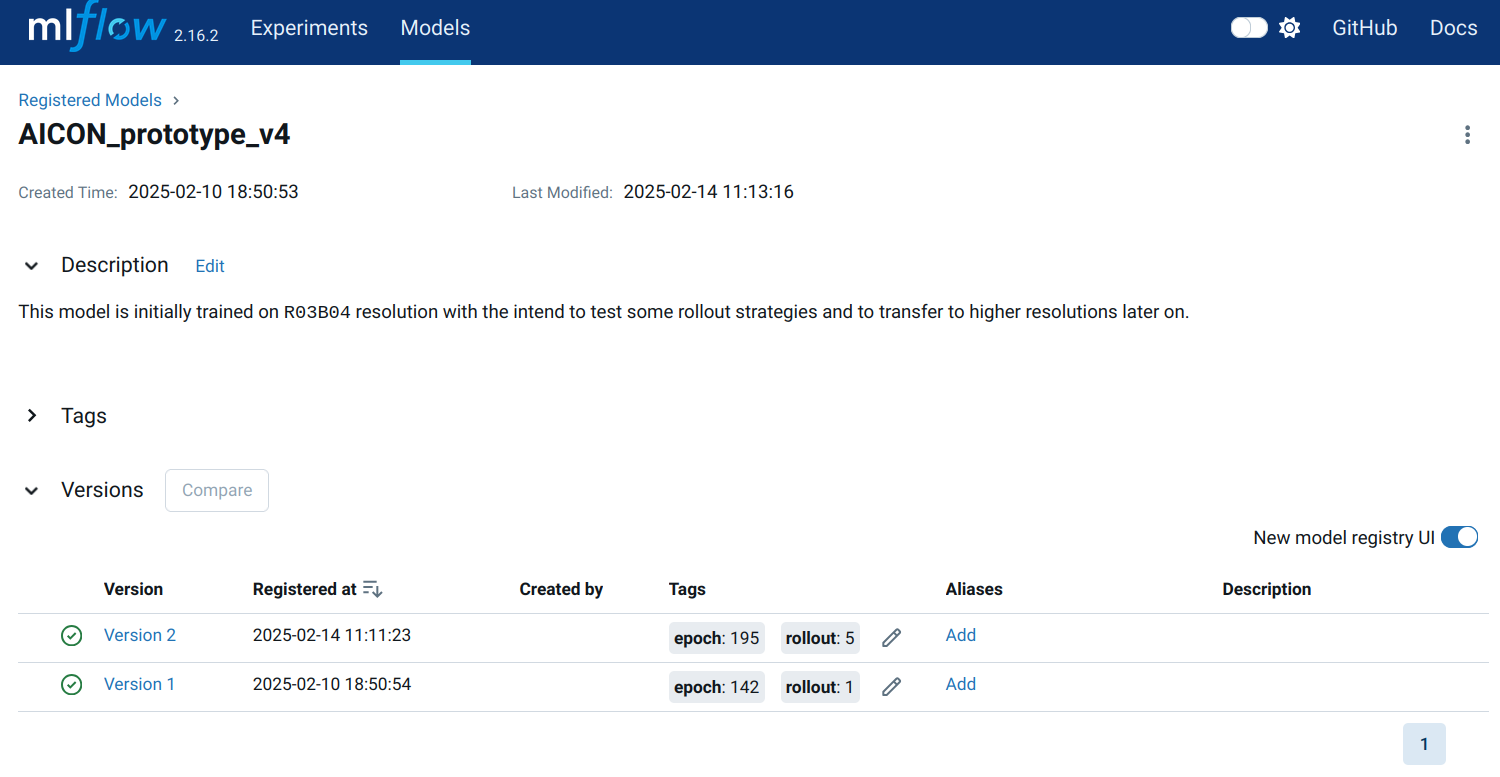
\includegraphics[width=0.85\textwidth]{images/mlflow_registry.png}
    \caption{MLFlow model registry.}
    \label{fig:mlflow_registry}
\end{figure}

\begin{figure}[htbp]
    \centering
    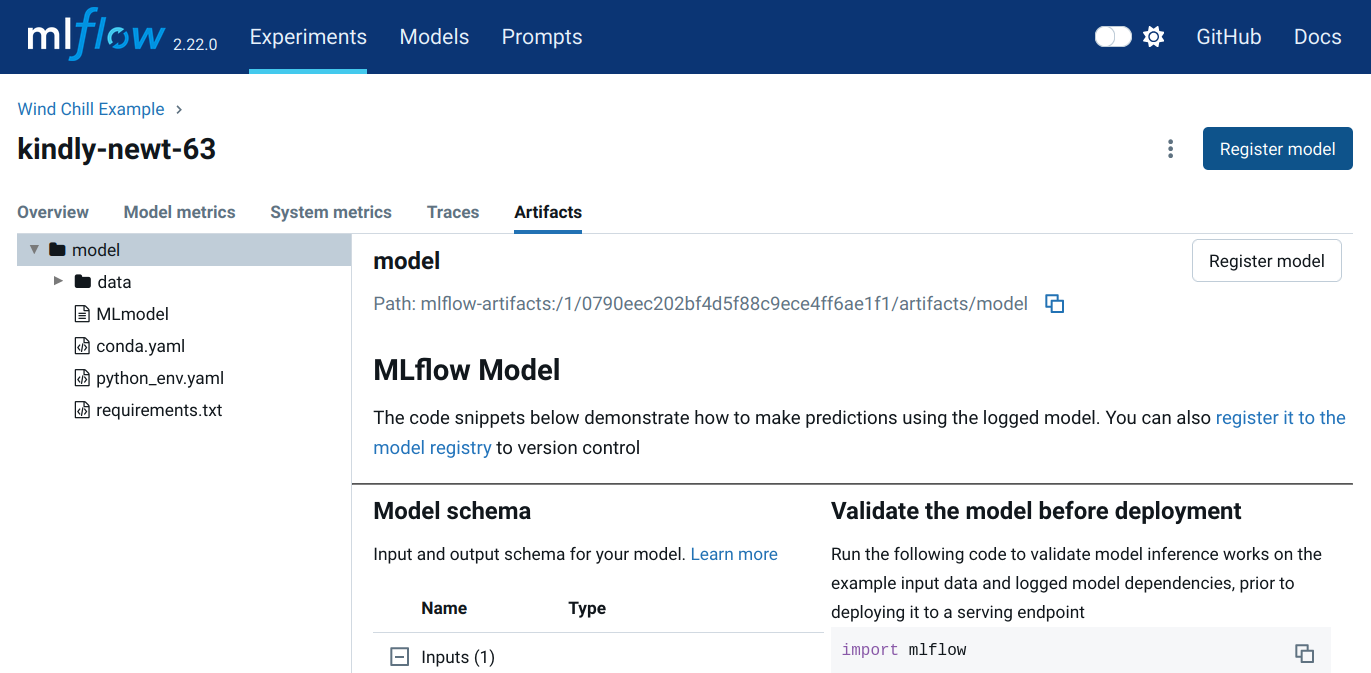
\includegraphics[width=0.85\textwidth]{images/mlflow_register.png}
    \caption{Register a model in MLFlow by first selecting the experiment run, and pressing the \textbf{Register model} button on the right.}
    \label{fig:mlflow_register}
\end{figure}

%------------------------------------------------------------------------------
%
%------------------------------------------------------------------------------
\subsection{Exporting and Importing Experiments}

To migrate experiments between MLFlow servers, you can use the \texttt{mlflow-export-import} plugin. Note that new (internal) run IDs are assigned by MLflow when importing an experiment.

This allows moving:
\begin{itemize}
    \item experiments from file-based runs to a central server
    \item runs from one MLFlow instance to another
\end{itemize}

\begin{codeonly}{Export Experiment}
pip install mlflow-export-import
export MLFLOW_TRACKING_URI=http://localhost:5000
export-experiment --experiment-name WindChill --output-dir /tmp/export
\end{codeonly}

\begin{codeonly}{Import Experiment}
export MLFLOW_TRACKING_URI=http://remote.server:5000
import-experiment --experiment-name WindChillCopy --input-dir /tmp/export
\end{codeonly}

Authentication (if enabled) can be passed via environment variables or URLs.


%------------------------------------------------------------------------------
%
%------------------------------------------------------------------------------
\subsection{Model Deployment and REST API}

MLFlow supports serving trained models through a REST API. Once a model is registered (Fig.~\ref{fig:mlflow_register} and promoted to production, it can be served like this:

\begin{codeonly}{Serve Model}
export MLFLOW_TRACKING_URI=http://localhost:5000 # required when serving from a MLflow server
mlflow models serve -m models:/modelfoo/latest --port 1234 --no-conda
\end{codeonly}

This starts a REST endpoint at \texttt{http://localhost:1234/invocations}, where clients can send input data via JSON. (Again, the \texttt{--host} options can be used to bind this service to the network.)

Example input format with 3 pairs of \texttt{tt, ff}:

\begin{codeonly}{Inference Request}
{
  "inputs": [[-5, 20], [0, 10], [10, 0]]
}
\end{codeonly}

You can use \texttt{curl}, Python requests, or Postman to test the model interface.

\begin{codeonly}{Inference Request Example with \texttt{curl}}
curl http://localhost:1234/invocations -H "Content-Type:application/json"  --data '{"inputs": [[-5, 20], [0, 10], [10, 0]]}'
\end{codeonly}

%------------------------------------------------------------------------------
%
%------------------------------------------------------------------------------
\subsection{MLFlow Recipes and Pipelines}

MLFlow Recipes (formerly known as MLFlow Pipelines) provide a declarative way to define reusable training workflows. These workflows follow a standard layout and are ideal for smaller problems with repeatable logic.

\begin{itemize}
    \item Steps: data loading, transformation, training, evaluation
    \item Each step is defined in YAML and Python
    \item Can be executed locally or remotely
\end{itemize}

\begin{codeonly}{Init Recipe}
mlflow recipes init classification --profile local
cd classification
mlflow recipes run
\end{codeonly}

%------------------------------------------------------------------------------
%
%------------------------------------------------------------------------------
\subsection{Summary}

In this section, we have seen how MLFlow supports:

\begin{itemize}
    \item Promoting and versioning models in a central registry
    \item Migrating experiments between systems
    \item Serving models as REST APIs
    \item Automating workflows using recipes
\end{itemize}

These capabilities are essential for moving from research to operational environments, ensuring reproducibility, traceability, and structured deployment.

The reader is kindly referd to the MLFlow documentation available online at \url{https://www.mlflow.org/docs}.